\documentclass{ctexart}
\usepackage{geometry}
\usepackage{fancyhdr}
\usepackage{graphicx}
\usepackage{booktabs}
\usepackage{amsmath}
\usepackage{tikz}
\usepackage{array}
\xeCJKsetup{CJKmath=true} 
\usepackage{zhnumber} % change section number to chinese
\renewcommand\thesection{\zhnum{section}}
\renewcommand \thesubsection {\arabic{subsection}}
\CTEXsetup[format={\Large\bfseries}]{section}

\geometry{
    a4paper,
    left=3.18cm,
    right=3.18cm,
    top=3.04cm,
    bottom=3.04cm
}

\pagestyle{fancy}
\fancyhf{}
\renewcommand{\headrulewidth}{0.7pt} % 设置页眉横线粗细
\fancyhead[L]{\kaishu\large 大学物理实验报告} % 在左侧设置页眉文字
\fancyhead[R]{\kaishu\large 哈尔滨工业大学(深圳) } % 在右侧设置页眉文字
\fancyfoot[R]{\thepage} % 将页数放在右下角


\setlength\headwidth{\textwidth}

\begin{document}

\noindent
\begin{center}
\textbf{
\begin{tabular}{p{2.4cm}p{2.4cm}p{4cm}p{4cm}}
    班级 \hrulefill & 学号 \hrulefill & 姓名 \hrulefill & 教师签字 \hrulefill \\
\end{tabular}
\begin{tabular}{p{6cm}p{3.6cm}p{3.6cm}}
    实验日期 \hrulefill & 预习成绩 \hrulefill & 总成绩 \hrulefill
\end{tabular}
{\noindent}	 \rule[-10pt]{\textwidth}{0.7pt}
}\end{center}

\begin{center}
    \Large \textbf{实验内容 \underline{空气中声速的测量}}
\end{center}

\section{实验预习}

相位比较法测量声速实验中,示波器上调出李萨如图形后,改变换能器的间距,连续记录出现正斜率和负斜率直线时接收器的位置(如下图所示),记录了10个位置数据xi(i=1, 2, 3, ……, 9, 10),所用声波频率为f,如下表所示,请用逐差法处理数据,推导出声速v的表达式。

\begin{figure}[h]
    \centering
    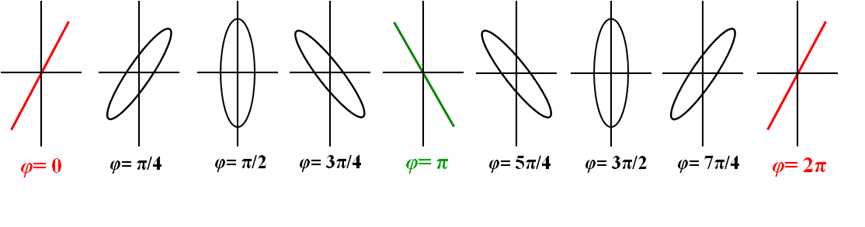
\includegraphics[width=\textwidth]{pic1.png} % 插入左侧图像
\end{figure}

\begin{table}[h]
    %\renewcommand\arraystretch{1.6}
    \centering
    \vspace{-0.8cm}
    \setlength{\belowcaptionskip}{-1cm}
    \begin{tabular}{|m{1.5cm}<{\centering}|m{0.7cm}<{\centering}|m{0.7cm}<{\centering}|m{0.7cm}<{\centering}|m{0.7cm}<{\centering}|m{0.7cm}<{\centering}|m{0.7cm}<{\centering}|m{0.7cm}<{\centering}|m{0.7cm}<{\centering}|m{0.7cm}<{\centering}|m{0.7cm}<{\centering}|}
        \hline
        次数& 1 & 2 & 3 & 4 & 5 & 6 & 7 & 8 & 9 & 10 \\ 
        \hline
        $l_i(mm)$& & & & & & & & & & \\
        \hline
    \end{tabular}
    \caption{相位比较法测空气中声速,频率$f = \rule{1.3cm}{0.4pt}$}
\end{table}

\newpage
\section{实验现象及原始数据记录}

\begin{table}[!h]
    %\renewcommand\arraystretch{1.6}
    \centering
    \caption{极值法(驻波法)测空气中声速,温度$t = \rule{1cm}{0.4pt} ^\circ C$,频率$f = \rule{1cm}{0.4pt} KHz$}
    \begin{tabular}{|m{1.5cm}<{\centering}|m{0.7cm}<{\centering}|m{0.7cm}<{\centering}|m{0.7cm}<{\centering}|m{0.7cm}<{\centering}|m{0.7cm}<{\centering}|m{0.7cm}<{\centering}|m{0.7cm}<{\centering}|m{0.7cm}<{\centering}|m{0.7cm}<{\centering}|m{0.7cm}<{\centering}|}
        \hline
        次数& 1 & 2 & 3 & 4 & 5 & 6 & 7 & 8 & 9 & 10 \\ 
        \hline
        $l_i(mm)$& & & & & & & & & & \\
        \hline
    \end{tabular}
\end{table}

\begin{table}[!h]
    %\renewcommand\arraystretch{1.6}
    \centering
    \caption{相位比较法测空气中声速,温度$t = \rule{1cm}{0.4pt} ^\circ C$,频率$f = \rule{1cm}{0.4pt} KHz$}
    \begin{tabular}{|m{1.5cm}<{\centering}|m{0.7cm}<{\centering}|m{0.7cm}<{\centering}|m{0.7cm}<{\centering}|m{0.7cm}<{\centering}|m{0.7cm}<{\centering}|m{0.7cm}<{\centering}|m{0.7cm}<{\centering}|m{0.7cm}<{\centering}|m{0.7cm}<{\centering}|m{0.7cm}<{\centering}|}
        \hline
        次数& 1 & 2 & 3 & 4 & 5 & 6 & 7 & 8 & 9 & 10 \\ 
        \hline
        $l_i(mm)$& & & & & & & & & & \\
        \hline
    \end{tabular}
\end{table}

\begin{table}[!h]
    %\renewcommand\arraystretch{1.6}
    \centering
    \caption{波形移动法测空气中声速,温度$t = \rule{1cm}{0.4pt} ^\circ C$,频率$f = \rule{1cm}{0.4pt} KHz$}
    \begin{tabular}{|m{1.5cm}<{\centering}|m{0.7cm}<{\centering}|m{0.7cm}<{\centering}|m{0.7cm}<{\centering}|m{0.7cm}<{\centering}|m{0.7cm}<{\centering}|m{0.7cm}<{\centering}|m{0.7cm}<{\centering}|m{0.7cm}<{\centering}|m{0.7cm}<{\centering}|m{0.7cm}<{\centering}|}
        \hline
        次数& 1 & 2 & 3 & 4 & 5 & 6 & 7 & 8 & 9 & 10 \\ 
        \hline
        $l_i(mm)$& & & & & & & & & & \\
        \hline
    \end{tabular}
\end{table}

\begin{table}[!h]
    %\renewcommand\arraystretch{1.6}
    \centering
    \caption{时差法测空气中声速,温度$t = \rule{1cm}{0.4pt} ^\circ C$}
    \begin{tabular}{|m{1.5cm}<{\centering}|m{0.7cm}<{\centering}|m{0.7cm}<{\centering}|m{0.7cm}<{\centering}|m{0.7cm}<{\centering}|m{0.7cm}<{\centering}|m{0.7cm}<{\centering}|m{0.7cm}<{\centering}|m{0.7cm}<{\centering}|m{0.7cm}<{\centering}|m{0.7cm}<{\centering}|}
        \hline
        次数& 1 & 2 & 3 & 4 & 5 & 6 & 7 & 8 & 9 & 10 \\ 
        \hline
        $x_i$& & & & & & & & & & \\
        \hline
        $t_i(\mu s)$& & & & & & & & & & \\
        \hline
    \end{tabular}
\end{table}

\begin{table}[!h]
    %\renewcommand\arraystretch{1.6}
    \centering
    \caption{时差法测固体中声速,温度$t = \rule{1cm}{0.4pt} ^\circ C$}
    \begin{tabular}{|m{1.5cm}<{\centering}|m{1.2cm}<{\centering}|m{1.2cm}<{\centering}|m{1.2cm}<{\centering}|m{1.2cm}<{\centering}|m{1.2cm}<{\centering}|m{1.2cm}<{\centering}|}
        \hline
        次数& 1 & 2 & 3 & 4 & 5 & 6  \\ 
        \hline
        材质& \multicolumn{3}{c|}{} & \multicolumn{3}{c|}{} \\
        \hline
        $x_i$& & & & & &  \\
        \hline
        $t_i(\mu s)$& & & & & & \\
        \hline
    \end{tabular}
\end{table}

\begin{tikzpicture}[remember picture,overlay]
    \node[anchor=south east,inner sep=100pt] at (current page.south east) {
        \renewcommand{\arraystretch}{1.5} % 表格行高倍数
        \setlength{\tabcolsep}{18pt}    
    \begin{tabular}{|c|c|}
        \hline
        \LARGE  教师 & \LARGE  姓名 \\
        \hline
        \LARGE \kaishu 签字 &  \\
        \hline
        \end{tabular}
    };
\end{tikzpicture}

\newpage

\section{数据处理}

【计算以上几种方法测得的声速,计算室温下空气中声速的理论值,分别计算四种方法得到的声速测量值与理论值的相对误差,根据时差法测量数据计算固体介质中的声速(选做),要有详细的计算过程,格式工整】

首先计算理论声速有:

$$ v_0 = 331.45\sqrt{1+\frac{22.7}{273.15}} = 344.95\ m/s $$

\subsection{极值法(驻波法)测空气中声速}

代入数据根据逐差法公式计算,此时频率为$ \ Hz$。测量时每出现一次振幅极值则记录一次数据,即两相邻数据之间间隔半个波长,可得: 

$$ \overline{\lambda} = \frac{\sum\limits_{i=1}^{5}(l_{i+5}-l_i)}{5 \times 2.5} $$
$$ v = \overline{\lambda} f $$
$$ \sigma = \frac{|v - v_0|}{v_0} $$
$$ \overline{\lambda} = 9.43 mm , v = 349.24 \ m/s,\sigma = 1.25\% $$

\subsection{相位比较法测空气中声速}

代入数据根据逐差法公式计算,此时频率为$ \ Hz$。测量时每出现一次直线则记录一次数据,即两相邻数据之间间隔半个波长,可得:

$$ \overline{\lambda} = \frac{\sum\limits_{i=1}^{5}(l_{i+5}-l_i)}{5 \times 2.5} $$
$$ v = \overline{\lambda} f $$
$$ \sigma = \frac{|v - v_0|}{v_0} $$
$$ \overline{\lambda} = 9.47 mm , v = 350.97 \ m/s,\sigma = 1.75\% $$

\subsection{波形移动法测空气中声速}

代入数据根据逐差法公式计算,此时频率为$ \ Hz$。测量时每出现一次相位重叠则记录一次数据,即两相邻数据之间间隔一个波长,可得: 

$$ \overline{\lambda} = \frac{\sum\limits_{i=1}^{5}(l_{i+5}-l_i)}{5 \times 5} $$
$$ v = \overline{\lambda} f $$
$$ \sigma = \frac{|v - v_0|}{v_0} $$
$$ \overline{\lambda} = 9.56 mm , v = 354.11 \ m/s,\sigma = 2.66\% $$

\subsection{时差法测空气中声速}

两相邻数据间隔变化$\Delta x = 10\ mm$,每次记录两参考点的时间差可得:

\subsubsection{速度逐差}

$$ \overline{v} = \frac{1}{5} \sum\limits_{i = 1}^{5} \frac{l_{i+5}-l_i}{t_{i+5}-t_i} $$
$$ \sigma = \frac{|v - v_0|}{v_0} $$
$$ \overline{v} = 346.72 \ m/s, \sigma = 0.51\% $$

\subsubsection{时间逐差}

$$ \overline{v} = \frac{\Delta x \cdot 5 \times 5}{\sum\limits_{i=1}^{5}(t_{i+5}-t_i)} $$
$$ \sigma = \frac{|v - v_0|}{v_0} $$
$$ \overline{v} = 346.26 \ m/s, \sigma = 0.38\% $$

两种计算方法相差不大,可取第一组结果为测量结果。

\subsection{(选做)时差法测固体中声速}

每个固体材料传声长为50mm,每次记录两参考点的时间差可得: 

有机玻璃:
$$ v_1 = \frac{l_2-l_1}{t_2-t_1} = 4902 \ m/s $$
$$ v_2 = \frac{l_3-l_2}{t_3-t_2} = 4310 \ m/s $$
$$ v_{avg1} = \frac{v_1+v_2}{2} = 4606 \ m/s $$

铝:
$$ v_3 = \frac{l_5-l_4}{t_5-t_4} = 2155 \ m/s $$
$$ v_4 = \frac{l_6-l_5}{t_6-t_5} = 2049 \ m/s $$
$$ v_{avg2} = \frac{v_1+v_2}{2} = 2102 \ m/s $$

\section{实验结论及现象分析}

四次针对空气中声速的测量结果的相对误差均位于$\sigma \leq 3\%$区间内,认为计算值与理论值相差不大。考虑到四次声速测量的测量值全部紧密地集中在这一区间,可以合理怀疑测量值与理论值的偏差来自测量存在系统误差或理论声速计算公式的适用条件与实际空气状态不完全符合。实际空气中存在例如水蒸气、尘埃等加速传声的物质,可能导致测量值出现偏差。 

极值法(驻波法)、相位法、波形移动法需要判断何时振幅到达极值、李萨如图何时成为直线,何时相位重叠。即使做了充足的准备工作,观察导致的误差也不容忽视,另外还需要已知声音频率。由于声音频率会随着发声设备的运行而变化,理论上这三种方法的误差都应较大。时差法不需要了解频率,原理简单,主观性不强且不需要做大量准备工作,但可能产生不容忽视误差的地方在于示波器的分辨率不足,测量时间时有效数字不够。

\section{讨论题}

\subsection{使用驻波法测声速时,为什么示波器上观察到的是正弦波而不是驻波?}

驻波是空间范畴内的概念,在两个换能器之间的声波可以近似视为驻波。而示波器测量的是接收换能器那一位置的波动随着时间的变化情况,测量的是时间范畴量。接收换能器位置的声压方程为:

$$ p = \rho_0 \omega \nu \left[(A_1-A_2)\sin\left(\frac{2\pi x}{\lambda}\right)\cos(\omega t)-(A_1+A_2)\cos\left(\frac{2\pi x}{\lambda}\right)\sin(\omega t)\right]  $$

认为$ A_2 \approx A_1 $ , 则接收换能器位置的声压方程具有驻波形式,为:

$$  p = -\rho_0 \omega \nu (A_1+A_2)\cos\left(\frac{2\pi x}{\lambda}\right)\sin(\omega t) $$

显然当换能器位置$x$一定时,产生的波形是正弦波。

\subsection{用相位比较法测量波长时,为什么用直线而不用椭圆作为S2移动距离的判断数据?}

直线的主观误差较小。椭圆是曲线,对其进行观察时主观误差更大,为减小此类误差应选择直线进行观察。

\subsection{分析一下本实验中哪些因素可以引起测量误差。列出3条主要因素并说明原因。}

1. 接收换能器位置的声压方程中认为$ A_2 \approx A_1 $,而实际未知。

2. 实验中极值法(驻波法)判断何时振幅到达极值、相位比较法判断李萨如图何时成为直线,波形移动法判断何时相位重叠均具有较强的主观性,误差应较大。

3. 实验环境中的空气不是理想气体,测量值应与理论值存在差距,各仪器随着工作,内部电特性会发生微小的变化,可能影响到波动的产生与测量。

\end{document}